\documentclass[department=ds, notes={hide notes}, slidesperpage=1]{beamerruhuisstijl}

% Force pretty font
\usepackage[utf8]{inputenc}
\usepackage[english]{babel}
\usepackage{lmodern}
\usepackage[T1]{fontenc}
\usepackage{textcomp}
\usepackage[babel=true]{microtype}

\title{Roerei}
\subtitle{
	Premise selection for Coq\\
	\\
	Wouter Geraedts
}

\date{\today}

\usepackage{color}
\definecolor{green}{rgb}{0.0,0.5,0.0}
\definecolor{red}{rgb}{0.5,0.0,0.0}
\definecolor{darkred}{rgb}{0.4,0.0,0.0}
\definecolor{purple}{rgb}{0.5,0.0,0.3}
\definecolor{darkviolet}{rgb}{0.58, 0.0, 0.83}
\definecolor{lightblue}{rgb}{0.1, 0.1, 0.9}
\definecolor{darkgreen}{rgb}{0.0, 0.2, 0.13}
\definecolor{darkblue}{rgb}{0.0, 0.4, 0.0}

\usepackage{xspace}

\usepackage[sc]{mathpazo}
\usepackage{amsthm}
\usepackage{algorithmic}
\usepackage{amsmath}
\usepackage{amssymb}

\usepackage{url}
\usepackage{hyperref}
\usepackage{glossaries}

\newcommand{\Ms}{Master's thesis\xspace}
\newcommand{\citationeeded}{[citation needed]}

% Generic
\newcommand{\machinelearning}{Machine Learning\xspace}
\newcommand{\crossvalidation}{cross validation\xspace}
\newcommand{\dagraph}{directed acyclic graph\xspace}
\newcommand{\premiseselection}{premise selection\xspace}
\newcommand{\Premiseselection}{Premise selection\xspace}

% Math
\newcommand{\nat}{\mathbb{N}}
\newcommand{\rat}{\mathbb{R}}

\newcommand{\powerset}[1]{\ensuremath{\mathcal{P}({#1})}}

\newcommand{\infimum}{\bot}
\newglossaryentry{infimum}{name={\ensuremath{\infimum}},
description={greatest element of a poset that is less than or equal to all elements of that poset}}

\newcommand{\nth}[2]{\text{nth}({#1}, {#2})}
\newglossaryentry{nth}{name={\ensuremath{\nth{n}{X}}},
description={the $n^{\text{th}}$ bottom element in a totally ordered set}}

\newcommand{\downset}[2]{~{#1}\downarrow{#2}~}
\newglossaryentry{downset}{name={\ensuremath{\downset{X}{x}}},
description={subset of a poset $X$ where each element is less than or equal to a given element $x$}}

% Lists
\newcommand{\listtype}[1]{\ensuremath{\mathcal{L}({#1})}}
\newcommand{\nil}{\ensuremath{\text{nil}}}
\newcommand{\cons}[2]{\ensuremath{\text{cons}({#1},~{#2})}}

\newcommand{\mapsymbol}{\ensuremath{\text{map}}}
\newcommand{\map}[2]{\ensuremath{\mapsymbol( {#1},~{#2})}}

\newcommand{\concatsymbol}{\ensuremath{\uplus}}
\newcommand{\concat}[2]{{#1} ~\concatsymbol~ {#2}}

\newcommand{\flattenlistsym}{\ensuremath{\text{flatten}}}
\newcommand{\flattenlist}[1]{\ensuremath{\flattenlistsym({#1})}}

\newcommand{\foldrsym}{\ensuremath{\text{foldr}}}
\newcommand{\foldr}[3]{\ensuremath{\foldrsym({#1},~ {#2},~ {#3})}}

\newcommand{\singleton}[1]{\ensuremath{[ {#1} ]}}

% Languages
\newcommand{\cpp}{C++\xspace}
\newcommand{\ocaml}{OCaml\xspace}
\newcommand{\python}{Python\xspace}
\newcommand{\matlab}{MATLAB\xspace}
\newcommand{\xml}{XML\xspace}
\newcommand{\msgpack}{\texttt{msgpack}\xspace}

% Projects
\newcommand{\preloader}{\texttt{preloader}\xspace}
\newcommand{\roerei}{\texttt{roerei}\xspace}
\newcommand{\coq}{Coq\xspace}
\newcommand{\coqide}{CoqIDE\xspace}

% Corpora
\newcommand{\compcert}{CompCert\xspace}
\newcommand{\corn}{CoRN\xspace}
\newcommand{\formalin}{Formalin\xspace}
\newcommand{\mathclasses}{Mathematical Classes\xspace}
\newcommand{\mathcomp}{Mathematical Components\xspace}
\newcommand{\ssreflect}{SSReflect\xspace}

% Machine learning methods
\newcommand{\knn}{$k$-Nearest Neighbor\xspace}
\newcommand{\knnadaptive}{Adaptive Nearest Neighbor\xspace}
\newcommand{\nb}{Naive Bayes\xspace}
\newcommand{\ensemble}{Ensemble Learning\xspace}
\newcommand{\omniscient}{Omniscient\xspace}
\newcommand{\mepo}{the MePo relevance filter\xspace}
\newcommand{\adarank}{Adarank\xspace}

% Coq terminology
\newcommand{\cprop}{\texttt{CProp}\xspace}

\newglossaryentry{termclass}{name={term},
description={a noun or compound word of \pcic, used by \gallina}}
\newglossaryentry{typeclass}{name={type},
description={the semantic subclass of types inside the syntactic class term}}
\newglossaryentry{sentence}{name={sentence},
description={a named term along with the corresponding type}}
\newglossaryentry{sort}{name={sort},
description={the type of a type when manipulated as term}}

\newcommand{\sorts}{\texttt{Sorts}\xspace}
\newglossaryentry{sorts}{name={\ensuremath{\sorts}}, sort=sorts,
description={the set of sorts}}
\newcommand{\sortprop}{\texttt{Prop}\xspace}
\newglossaryentry{sortprop}{name={\sortprop}, sort=prop,
description={the type of logical propositions}}
\newcommand{\sortset}{\texttt{Set}\xspace}
\newglossaryentry{sortset}{name={\sortset}, sort=set,
description={the type of small sets}}
\newcommand{\sorttype}[1][]{\texttt{Type}\ifthenelse{\equal{#1}{}}{}{({#1})}\xspace}
\newglossaryentry{sorttype}{name={\sorttype},
description={the type of types}}

\newcommand{\cic}{Cic\xspace}
\newglossaryentry{cic}{name={\cic},
description={Calculus of (Co)Inductive Constructions}}

\newcommand{\acic}{aCic\xspace}
\newglossaryentry{acic}{name={\acic},
description={Calculus of (Co)Inductive Constructions with Explicit Named Substitutions}}

\newcommand{\pcic}{pCic\xspace}
\newglossaryentry{pcic}{name={\pcic},
description={Predicative Calculus of (Co)Inductive Constructions}}

\newcommand{\gallina}{Gallina\xspace}
\newglossaryentry{gallina}{name={\gallina},
description={the specification language for \coq}}

% Paper-bound definitions
\newcommand{\coqobj}[1][]{\coq object\ifthenelse{\equal{#1}{}}{}{~${#1}$}\xspace}
\newcommand{\coqobjs}{\coq objects\xspace}
\newglossaryentry{coqobj}{name={\coqobj[s]},
description={an object defined in \coq. Might be an inductive type, an axiom or a proof}}

\newglossaryentry{theorem}{name=theorem,
description={\coqobjs that have been proved based on previously established \coqobjs}}

\newglossaryentry{definition}{name=definition,
description={\coqobjs that are not theorems. Either simple constants or purely transformative operations on such constants}}

\newcommand{\name}[1][]{n_{#1}}
\newglossaryentry{name}{name={\ensuremath{\name[s]}},
description={canonical form of the name of the \coqobj[s]}}

\newcommand{\names}{\mathcal{N}}
\newglossaryentry{names}{name={\ensuremath{\names}},
description={the set of all names}}

\newcommand{\term}[1][]{t_{#1}}
\newglossaryentry{term}{name={\ensuremath{\term[s]}},
description={term of the \coqobj[s]}}

\newcommand{\terms}{\mathcal{T}}
\newglossaryentry{terms}{name={\ensuremath{\terms}},
description={the set of all terms}}

\newcommand{\emptyterm}{\top}
\newglossaryentry{emptyterm}{name={\ensuremath{\emptyterm}}, sort=term-empty,
description={the empty term}}

\newcommand{\type}[1][]{A_{#1}}
\newglossaryentry{type}{name={\ensuremath{\type[s]}},
description={type of the \coqobj[s]}}

\newcommand{\types}{\mathcal{A}}
\newglossaryentry{types}{name={\ensuremath{\types}},
description={the set of all types}}

\newcommand{\flattensym}{\nabla}
\newcommand{\flatten}[1]{\flattensym({#1})}
\newglossaryentry{flatten}{name={\ensuremath{\flattensym}}, sort=flatten,
description={extracts names from term or type, and return the set of names}}

\newcommand{\countsym}{\#}

\newcommand{\countoccursym}{\flattensym_\countsym}
\newcommand{\countoccur}[1]{\countoccursym({#1})}
\newglossaryentry{countoccur}{name={\ensuremath{\countoccursym}}, sort=flatten-countoccur,
description={extracts names from term or type along with their number of occurances}}

\newcommand{\depthsym}{D}

\newcommand{\depthoccursym}{\flattensym_\depthsym}
\newcommand{\depthoccur}[1]{\depthoccursym({#1})}
\newglossaryentry{depthoccur}{name={\ensuremath{\depthoccursym}}, sort=flatten-depthoccur,
description={extracts names from term or type along with their depth}}

\newcommand{\termset}[1]{\flatten{\term[#1]}}
\newglossaryentry{termset}{name={\ensuremath{\termset{s}}}, sort=flatten-termset,
description={set of names of all objects in the term of \coqobj[s]}}

\newcommand{\typeset}[1]{\flatten{\type[#1]}}
\newglossaryentry{typeset}{name={\ensuremath{\typeset{s}}}, sort=flatten-typeset,
description={set of names of all objects in the type of \coqobj[s]}}

\newcommand{\defs}[1][]{\texttt{Defs}_{#1}}
\newglossaryentry{defs}{name={\ensuremath{\defs}},
description={set of names of all objects in the types of all objects; used as the base of the set of features}}
\newcommand{\thms}[1][]{\texttt{Thms}_{#1}}
\newglossaryentry{thms}{name={\ensuremath{\thms}},
description={set of names of all objects in the terms of all objects, excluding all $\defs$; used as set of dependencies}}

% Metrics
\newcommand{\oocover}{100Cover\xspace}
\newcommand{\oocoverf}[2]{\ensuremath{\text{100Cover}({#1}, {#2})}}
\newcommand{\ooprecision}{100Precision\xspace}
\newcommand{\ooprecisionf}[2]{\ensuremath{\text{100Precision}({#1}, {#2})}}
\newcommand{\recall}{Recall\xspace}
\newcommand{\recallf}[2]{\ensuremath{\text{Recall}({#1}, {#2})}}
\newcommand{\rank}{Rank\xspace}
\newcommand{\rankf}[2]{\ensuremath{\text{Rank}({#1}, {#2})}}
\newcommand{\auc}{AUC\xspace}
\newcommand{\aucf}[2]{\ensuremath{\text{AUC}({#1}, {#2})}}
\newcommand{\volume}{Volume\xspace}

% Features
\newcommand{\featurekeys}{Z}
\newglossaryentry{featurekeys}{name={\ensuremath{\featurekeys}},
description={set of feature keys, or the set of the aspects with which an object can be described; based on the set of definitions $\defs$, but possibly extended with other aspects}}

\newcommand{\features}[2]{F^{#1}_{#2}}
\newglossaryentry{features}{name={\ensuremath{\features{}{}}},
description={function which computes the numeric values describing a \coqobj. These values are considered to be the features of the \coq object}}

\newcommand{\depsym}{D}

\newcommand{\deps}[1]{\depsym_{#1}}
\newglossaryentry{deps}{name={\ensuremath{\deps{s}}},
description={set of names of objects which have been used to define or prove a \coqobj $s$}}

\newcommand{\depset}{\depsym}
\newglossaryentry{depset}{name={\ensuremath{\depset}},
description={set of all possible dependencies}}

\newcommand{\depstrans}[1][]{\deps{#1}^*}

\newcommand{\parentsym}{P}

\newcommand{\parents}[1][]{\parentsym_{#1}}
\newglossaryentry{parentsym}{name={\ensuremath{\parents{s}}},
description={set of names of objects which use \coqobj $s$ to be defined to or proven}}

\newcommand{\parentstrans}[1][]{\parents[{#1}]^*}

% Predictors
\newcommand{\predictors}{\mathcal{P}}
\newglossaryentry{predictors}{name={\ensuremath{\predictors}},
description={set of predictor functions}}

\newcommand{\rankings}{\mathcal{R}}
\newglossaryentry{rankings}{name={\ensuremath{\rankings}},
description={set of rankings}}

\newcommand{\dist}{\text{dist}}
\newglossaryentry{dist}{name={\ensuremath{\dist}},
description={the euclidean distance between two types $a, b \in \types$ computed using the features $\features{}{a}$ and $\features{}{b}$ of those types}}

\newcommand{\objsym}{\ensuremath{S}}
\newcommand{\objs}[1][]{\ensuremath{\objsym_{#1}}}
\newcommand{\trainset}{\objs[{\text{train}}]}
\newcommand{\testset}{\objs[{\text{test}}]}

\newcommand{\objdef}{:=}

\newcommand{\findindex}[2]{\ensuremath{i}({#1}, {#2})}
\newcommand{\firstsym}{\ensuremath{\text{first}}}
\newcommand{\topn}[2]{\ensuremath{\mathtt{top}_{#1}({#2})}}
\newcommand{\required}[1][]{\ensuremath{{\mathtt{req}}_{#1}}}
\newcommand{\suggestions}[1]{\ensuremath{\mathtt{sugg}_{#1}}}

\newcommand{\ltr}{\emph{Learning to rank}\xspace}

% Adarank

\newcommand{\query}{\ensuremath{q}}
\newcommand{\doc}{\ensuremath{d}}
\newcommand{\docs}[1]{\ensuremath{\mathbf{d}_{#1}}}
\newcommand{\queries}{\ensuremath{Q}}
\newcommand{\rankdoc}[1]{\ensuremath{y}_{#1}}
\newcommand{\irfeatures}{\ensuremath{\mathcal{X}}}

\newcommand{\idf}{\ensuremath{\mathbf{idf}}}


\usepackage{tikz}
\usepackage{tabularx}
\usepackage{prooftree}

\usepackage{pgfplots}
\usepackage{pgfplotstable}

\usepackage{bibentry}

\usepackage{listings}
\usepackage{prettylistings}
\usepackage{lang-coq}

\begin{document}
\renewcommand{\dept}{icis}

\bibliographystyle{plain}

% Load literature in temporary savebox to prevent generation of new frame
\newsavebox\mytempbib
\savebox\mytempbib{\parbox{\textwidth}{\nobibliography{literature}}}

\begin{frame}
	\titlepage
\end{frame}

\begin{frame}{Outline}
	\begin{itemize}
		\item Background: what is Premise Selection?
		\item Approach: how to do ATP for Coq?
		\item Contributions
		\item Showcase: adaptation of Learning to Rank
		\item Results
	\end{itemize}
\end{frame}

\begin{frame}{Proofs}
	\begin{minipage}{0.5\textwidth}
		\begin{itemize}
			\item All men are mortal.
			\item Socrates is a man.
			\item Therefore, Socrates is mortal.
		\end{itemize}
	\end{minipage}
	\hspace{2em}
	\begin{minipage}{0.4\textwidth}
		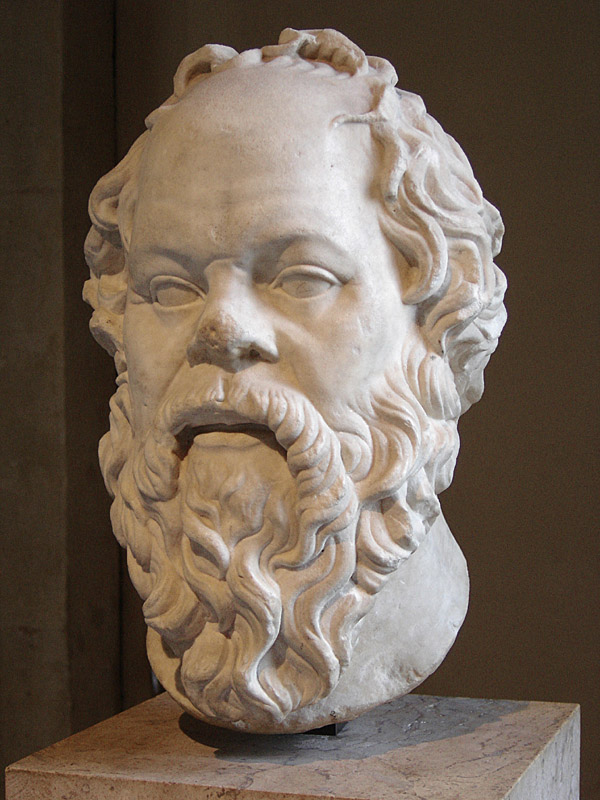
\includegraphics[width=1.0\textwidth]{figures/socrates.jpg}\\
		\centering \color{gray}{Eric Gaba (CC by-nc-sa 2.5)}
	\end{minipage}
\end{frame}

\begin{frame}{Propositional logic}
	\begin{block}{Primitives}
			Atomic values: $P, Q$\\
			Operations: $\rightarrow$\\
			Term: $P \rightarrow Q$\\
			Derivation: $H_1, \dots, H_n \vdash P$
	\end{block}

	\uncover<2->{
	\begin{block}{Proof rules}
			\begin{center}
					\begin{minipage}{.4\textwidth}
					\[
							\begin{prooftree}
									\justifies
									H, P \vdash P
									\using \text{hyp}
							\end{prooftree}
					\]
					\end{minipage}
					\begin{minipage}{.4\textwidth}
							\[
									\begin{prooftree}
											H, P \vdash Q
											\justifies
											H \vdash P \rightarrow Q
											\using \rightarrow \text{intro}
									\end{prooftree}
							\]
					\end{minipage}\\
					\vspace{1em}
					\begin{minipage}{1.0\textwidth}
					\[
							\begin{prooftree}
											H, \vdash P \rightarrow Q
											\hspace{1em}
											H \vdash P
											\justifies
											H \vdash Q
											\using \rightarrow \text{elim}_{[P]}
							\end{prooftree}
					\]
					\end{minipage}
			\end{center}
	\end{block}
	}
\end{frame}

\begin{frame}{Propositional logic \small{example}}
	\begin{block}{Theorem}
			\[ (P \rightarrow Q) \rightarrow P \rightarrow Q \]
	\end{block}
	\begin{block}{Proof}
			\[
					\begin{prooftree}
							\begin{prooftree}
									\begin{prooftree}
											\justifies
											P \rightarrow Q, \dots \vdash P \rightarrow Q
											\using \text{hyp}
									\end{prooftree}
									\hspace{1em}
									\begin{prooftree}
											\justifies
											\dots, P \vdash P
											\using \text{hyp}
									\end{prooftree}
									\justifies
									P \rightarrow Q, P \vdash Q
									\using \rightarrow \text{elim}_{[P]}
							\end{prooftree}
							\justifies
							\vdash (P \rightarrow Q) \rightarrow P \rightarrow Q
							\using \rightarrow \text{intros}
					\end{prooftree}
			\]
	\end{block}
\end{frame}

\begin{frame}{Automated Theorem Proving}
	For a (unproven) theorem, find proof consisting of these proof steps.\\
	\bigskip
	\begin{itemize}
		\item Premise selection: finding useful theorems
		\item Proof construction: applying steps
		\item Proof verification: checking correctness
	\end{itemize}
	\bigskip
	First ATP guided proof: Davis, 1957.
\end{frame}

\begin{frame}{Successes of Automated Theorem Proving}
	\begin{block}{Kepler Conjecture}
		What is the best way to stack cannonballs?
		\bigskip
		\begin{center}
				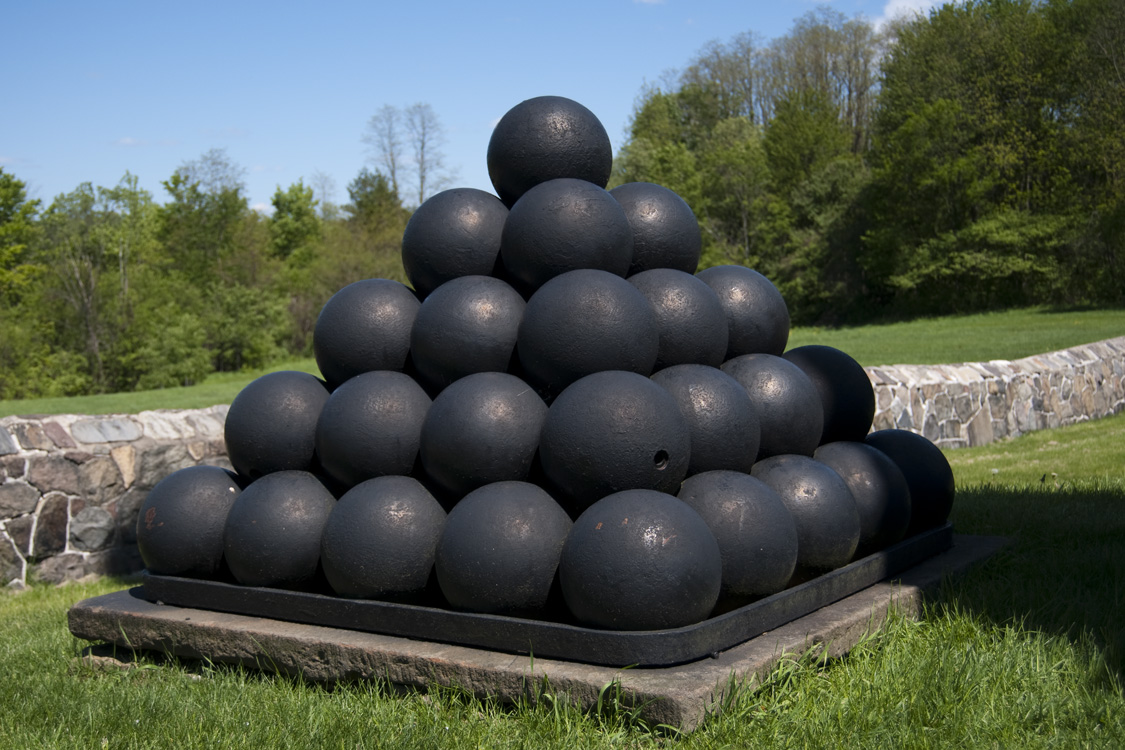
\includegraphics[width=0.5\textwidth]{figures/balls.jpg}\\
				\centering \color{gray}{Nedral (CC by-nc-sa 2.5)}
		\end{center}
		
		\small{
				No arrangement of equally sized spheres has a greater average than $\frac{\pi}{3\sqrt{2}}$.
				Formalized in 2014 by Flyspeck using Isabelle and HOL Light.
		}
	\end{block}
\end{frame}

\begin{frame}{Interactive Theorem Proving}
	\begin{center}
		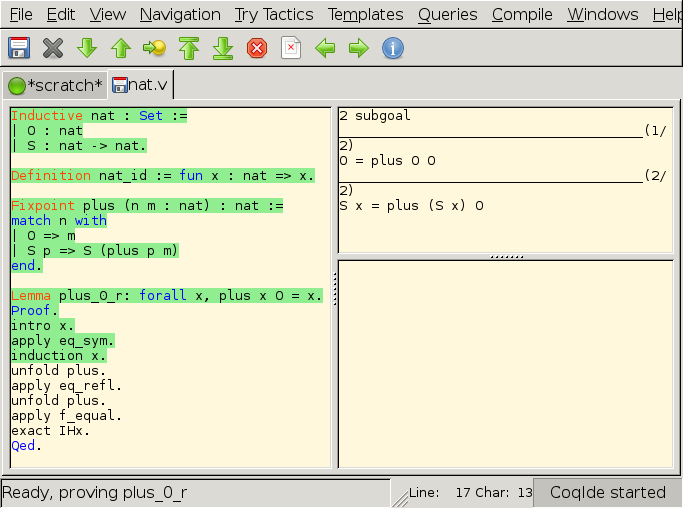
\includegraphics[height=0.78\textheight]{figures/coqide.png}
	\end{center}
\end{frame}

\begin{frame}{Premise Selection in ITP}
	\begin{center}
		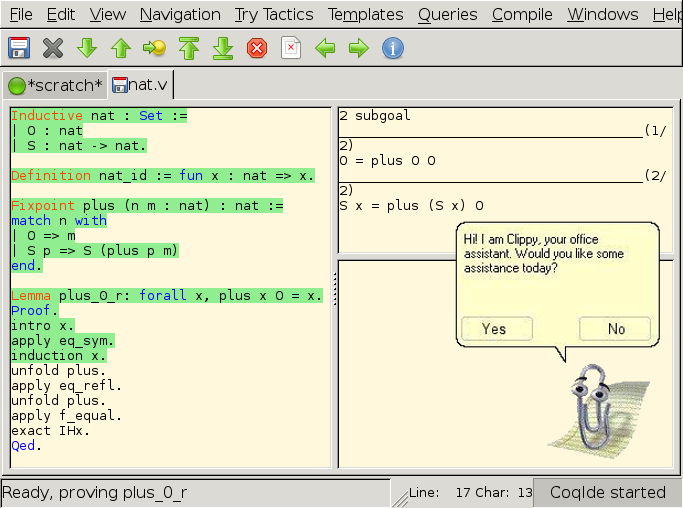
\includegraphics[height=0.78\textheight]{figures/coqide-clippy.png}
	\end{center}
\end{frame}

\begin{frame}{Source research}
	\begin{center}
		\bibentry{kaliszyk2014machine}
	\end{center}
\end{frame}

\begin{frame}{Roerei}
	Open source and is available from:
	\begin{center}
		\url{https://github.com/Wassasin/roerei}
	\end{center}
	\bigskip
	Design goals of this tool were to:
	\begin{itemize}
		\item Support offline learning and analysis of \machinelearning on the various corpora.
		\item Enable integration in the \coqide GUI.
		\item Enable merging of the premise selection tool in the \coq main branch as a plugin.
	\end{itemize}
\end{frame}

\begin{frame}[fragile]{Gallina}
\begin{lstlisting}[language=Coq, mathescape,basicstyle=\footnotesize,frame=none]
Inductive nat : Set :=
| O : nat
| S : nat -> nat.
Fixpoint plus (n m : nat) : nat :=
match n with
| O => m
| S p => S (plus p m)
end.
Lemma plus_0_r : $\forall$ x , plus x 0 = x.
Proof.
intro x.
apply eq_sym.
induction x.
unfold plus.
apply eq_refl.
unfold plus.
apply f_equal.
exact IHx.
Qed.
\end{lstlisting}
\end{frame}

\begin{frame}{\pcic: terms}
	Language on which \coq operates internally.\\
	\bigskip
	\begin{definition}[term]
		A term is a noun or compound word of \pcic.
		A term is typically denoted by $\term$,
		with $\terms$ being the set of all terms.
	\end{definition}
	\bigskip
	\begin{definition}[name]
		A name is an element in the set of names $\names$, and is bound to a term.
	\end{definition}
\end{frame}

\begin{frame}{\pcic: types}

	\begin{definition}[type]
		A type is denoted by the semantic subclass of types inside the syntactic class term.
		A type is typically denoted by $\type$, with $\types$ being the set of all types.
	\end{definition}
	\bigskip
	\begin{lemma}
	\coq is based on the Curry-Howard isomorphism.
	Therefor a type is inside the syntactic class term, and all types can also be considered to be terms.
	\[ \types \subseteq \terms \]
	\end{lemma}
\end{frame}

\begin{frame}{\pcic: sorts}
	\begin{definition}[sort]
		The type of a type when manipulated as a term is called a sort.
		\pcic uses an infinite well-founded typing hierarchy of sorts,
		with base sorts \sortprop and \sortset,
		and with a family of sorts \sorttype[{i}].
		The set of sorts named $\sorts$ is defined by
		\[\sorts \equiv \{ \sortprop, \sortset, \sorttype[{i}] ~|~ i \in \mathbb{N} \} \]
	
		Their types are defined as
		\[
			\rowcolors{0}{}{}
			\begin{array}{rcl}
				\sortprop & : & \sorttype[1] \\
				\sortset & : & \sorttype[1] \\
				\forall_{i \in \mathbb{N}}~ \sorttype[i] & : & \sorttype[{i+1}]
			\end{array}
		\]
	\end{definition}
\end{frame}

\begin{frame}{\pcic: example}
From our natural numbers example the following terms are of sort \sortset:
$$
	\rowcolors{0}{}{}
	\begin{array}{rcl}
		\texttt{0} & : & \texttt{nat} \\
		\texttt{S} & : & \texttt{nat} \rightarrow \texttt{nat}
	\end{array}
$$
$$
	\rowcolors{0}{}{}
	\begin{array}{rclcl}
		\texttt{nat\_id} & \objdef & \lambda x : \texttt{nat}~.~x & : & \texttt{nat} \rightarrow \texttt{nat} \\
		\texttt{plus} & \objdef & \texttt{fix}~\ldots & : & \texttt{nat} \rightarrow \texttt{nat} \rightarrow \texttt{nat} \\
	\end{array}
$$
\end{frame}

\begin{frame}{\pcic: example}
From our natural numbers example the following terms are of sort \sortprop:
$$
	\rowcolors{0}{}{}
	\begin{array}{rcl}
		\texttt{nat\_ind} & \objdef & \lambda~P~f_0~f_S ~.~ \texttt{fix}~F~n ~:~ P~n ~:= \\
			&   &  \texttt{match}~ n ~\texttt{with} \\
			&   &  ~~| ~0 => f_0 \\
			&	&  ~~| ~S~m => f_S~m~(F~m) \\
			&	&  \texttt{end} \\
			& : &  \forall P : \texttt{nat} \rightarrow \sortprop,\\
			&   & P~\texttt{0} \rightarrow (\forall n : \texttt{nat},~ P~n \rightarrow P~(\texttt{S}~n)) \rightarrow \forall n : \texttt{nat},~ P~n \\
		\\
		\texttt{plus\_0\_r} & \objdef & \texttt{eq\_sym}
							~~(\texttt{nat\_ind}~(\lambda x~.~\texttt{plus}~x~0)\\
							& & \texttt{eq\_refl}~(\lambda x~\texttt{IH}~.~\texttt{f\_equal}~S~\texttt{IH})~x) \\
							& : & \forall x : \texttt{nat},~ \texttt{plus}~x~0 = x \\
	\end{array}
$$
\end{frame}

\begin{frame}{\pcic: terms}
	\vspace{-0.7em}
	\begin{tabular}{ll}
		$\emptyterm$                                        & Empty term \\
		$\text{Rel}(i:\nat)$                       & Variables as De Bruijn index \\
		$\text{Var}(n:\names)$                     & Named (local) variables \\
		$\text{Evar}(xs:\listtype{\terms}) $        & Existential quantification \\
		$\text{Sort}(n:\names)$                    & Named Sort of types \\
		$\text{Cast}(t:\terms,~ A:\types)$ & Type casting check \\
		$\text{Prods}(x:\names,~ A:\types,~ B:\types$ & $\prod x:A ~.~ B$ \\
		$\text{Lambdas}(x:\names,~ A:\types,~ t:\terms)$   & $\lambda x:A ~.~ t$ \\
		$\text{LetIns}(n:\names,~ t:\terms,~ A:\types)$    & $\text{let~} n := t : A \text{~in~} t$ \\
		$\text{App}(x:\terms,~ ys:\listtype{\terms})$ & Application $x~ys_0 \ldots ys_n$ \\
		$\text{Const}(n:\names,~ S:\sorts)$ & Constant \\
		$\text{Ind}(n:\names,~ S:\sorts)$  & Inductive definition \\
		$\text{Construct}(n:\names,~ S:\sorts)$ & Constructor (of ind. def.) \\
		$\text{Case}(n:\terms,~ t:\terms,~ ys:\listtype{\terms})$ & Deconstruction (of ind. types) \\
		$\text{Fix}(n:\listtype{\names},~ A:\listtype{\types},~ ts:\listtype{\terms})$ & Fixpoint functions \\
		$\text{CoFix}(n:\listtype{\names},~ AS:\listtype{\types},~ ts:\listtype{\terms})$ & Co-fixpoint functions \\
	\end{tabular}
\end{frame}

\begin{frame}{\pcic: objects}
	\begin{tabular}{l}
		$\text{Constant}(n:\names,~ t:\terms,~ A:\types)$ \\
		$\text{Variable}(n:\names,~ t:\terms,~ A:\types)$ \\
		$\text{CurrentProof}(n:\names,~ \text{hyps}:\listtype{\listtype{\types} \times \terms}, t:\terms, A:\types)$ \\
		$\text{InductiveConstructor}(n:\names,~ A:\types)$ \\
		$\text{InductiveDefinition}(n:\names,~ A:\types,~ cs:\listtype{\text{InductiveConstructor}})$
	\end{tabular}
\end{frame}

\begin{frame}{\xml}
	\lstinline{COQ_XML=-xml COQ_XML_LIBRARY_ROOT=<dest>}
	\lstinputlisting[language=xml,basicstyle=\tiny]{figures/plus.con.xml}
\end{frame}

\begin{frame}{Parsing}
	\lstinputlisting[language=caml,basicstyle=\tiny]{figures/plus.con.types.txt}
\end{frame}

\begin{frame}{Extraction}
	\vspace{-2.55em}
	\[c : \terms \rightarrow \nat \rightarrow \listtype{\names \times \nat} \]
	\bigskip
	\hspace{-1.7em}
	\begin{tabularx}{\textwidth}{ll}
		$c(\emptyterm, d)$              & $ = \nil $ \\
		$c(\text{ARel}(\cdots), d)$     & $ = \nil $ \\
		$c(\text{AVar}(u), d)$          & $ = \singleton{(u, d)} $ \\
		$c(\text{AEvar}(l), d)$         & $ = \flattenlist{\map{l}{\lambda x . c(x, d+1)}} $ \\
		$c(\text{ASort}(\cdots), d)$    & $ = \nil $ \\
		$c(\text{ACast}(t, A), d)$      & $ = \concat{c(t, d+1)}{c(A, d+1)} $ \\
		$c(\text{AProds}(l, t), d)$     & $ = c_{\times}(l, t, d) $ \\
		$c(\text{ALambdas}(l, t), d)$   & $ = c_{\times}(l, t, d) $ \\
		$c(\text{ALetIns}(l, t), d)$    & $ = c_{\times}(l, t, d) $ \\
		$c(\text{AApp}(l), d)$  & $ = \left(
		  \begin{array}{l}
			\singleton{(\text{special:app}, d)} ~\concatsymbol \\
			\map{l}{ \lambda a . c(a, d+1) }
		  \end{array}
		  \right)
		  $ \\
		$c(\text{AConst}(\cdots, u), d)$  & $ = \singleton{(u, d)} $ \\
		$c(\text{AInd}(\cdots, u), d)$  & $ = \singleton{(u, d)} $ \\
		$c(\text{AConstruct}(\cdots, u), d)$  & $ = \singleton{(u, d)} $ \\
		$c(\text{ACase}(u, A, i, l), d)$  &
		  $= \left(
			\begin{array}{l}
			  \concat{\singleton{(u, d)}}{
				\concat{c(A, d+1)}{c(i, d+1)}
			  }
			  ~\concatsymbol \\
			  \flattenlist{ \map{l}{\lambda x . c(x, d+1)} } \\
			\end{array}
			\right)
		  $ \\
		$c(\text{AFix}(l), d)$        & $ = c_{\text{fix}}(l, d) $ \\
		$c(\text{ACoFix}(l), d)$      & $ = c_{\text{fix}}(l, d) $ \\
	\end{tabularx}
\end{frame}

\begin{frame}{Extraction}
	$$
		\rowcolors{0}{}{}
		\begin{array}{lcl}
		c_{\times}(l, t, d) & = &
			c(t, d+1) ~\concatsymbol \\
			& & \map{l}{ \lambda (n, a) ~.~ \cons{(\text{special:prod}, d)}{c(a, d+1)}} \\
		c_{\text{fix}}(l, d) & = & \flattenlist{ \map{l}{ \lambda (A, t) ~.~ \concat{c(A, d+1)}{c(t, d+1)} } }
		\end{array}
	$$
\end{frame}

\begin{frame}{Extraction}
	\hspace{-1em}\vbox{\begin{tabular}{ll}
		$c_{\text{type}}(\text{AConstant}(n, A, t))$ & $= c(A, 0)$ \\
		$c_{\text{type}}(\text{AIndDef}(n, l))$ & $= \flattenlist{
			\map{l}{
				\hspace{-0.5em}\begin{array}{l}
					\lambda (A, m) ~.~ c(A, 0) ~\concatsymbol\\
					\flattenlist{\text{map}(m, \lambda x . c(x, 0))}
				\end{array}
			}
		} $\\
		$c_{\text{type}}(-)$ & $= \nil $ \\
		$c_{\text{term}}(\text{AConstant}(n, A, t))$ & $= c(t, 0)$ \\
		$c_{\text{term}}(-)$ & $= \nil $ \\
	\end{tabular}}
\end{frame}

\begin{frame}{Counting}
	\[ \flattensym : \terms \rightarrow 2^{\names} \]
	\[ \flatten{t} = \foldr{\lambda (n, d)~s ~.~ \{n\} \cup s}{\varnothing}{c(t, 0)} \]
\end{frame}

\begin{frame}{Counting}
	\[ \countoccursym : \terms \rightarrow \nat^{\names} \]
	\[ \countoccur{t} = \lambda n ~.~ \foldr{\lambda (m, d)~s ~.~ \text{if~} n = m \text{~then~} s+1 \text{~else~} s}{0}{c(t, 0)} \]
	\bigskip
	\[ \depthoccursym : \terms \rightarrow \names \rightharpoonup \nat \]
	\[
		\rowcolors{0}{}{}
		\begin{array}{l}
		\depthoccur{t} = \lambda n ~.~ \foldr{\lambda (m, d)~s ~.~ \text{if~} n = m \text{~then~} f(d, s) \text{~else~} s}{\infimum}{c(t, 0)} \\
		\\
		\text{with~} \begin{array}{l}
			f(d, \infimum) = d \\
			f(d, s) = \text{min}(d, s) \\
		\end{array}
		\end{array}
	\]
\end{frame}

\begin{frame}{Theorems and definitions}
	\begin{definition}[Theorem]
		A type that has been proven, along with the term that proves it.
	\end{definition}
	\bigskip
	\begin{definition}[Definition]
		A term (which has a type) that is not a theorem.
		Thus it can only be transformative or a simple constant.
	\end{definition}
\end{frame}

\begin{frame}[fragile]{Theorems and definitions}
	\coq has a sort for theorems: \sortprop.
	\pause
	\bigskip
\begin{lstlisting}[language=Coq, mathescape]
Notation "'CProp'" := Type.
\end{lstlisting}
	\bigskip
	Thus for \corn the sort of a theorem is \sorttype{}$(n+1)$.
\end{frame}

\begin{frame}{Heuristic}
	Premise: a theorem concerning theorems in \coq is not useful.
	\bigskip
	\begin{definition}[$\defs$]
		All names occuring in types cannot be theorems, and thus must be definitions.
		\[ \defs = \bigcup_{s \in \objs} \typeset{s} \]
	\end{definition}
	\bigskip
	\begin{definition}[$\thms$]
		Theorems build upon eachother, thus what is used in terms, except the definitions, must be theorems.
		\[ \thms = (\bigcup_{s \in \objs} \termset{s}) \setminus \defs \]
	\end{definition}
\end{frame}

\begin{frame}{Features and dependencies}
	We are going to do machine learning, thus we need to define our dataset.
	\bigskip
	\begin{definition}[Features]
		For object $s$ yield whether definition $x \in \defs$ is used in the type of $s$.
		\[ \features{}{s}(x) = \flatten{\type[s]}(x) \]
	\end{definition}
	\bigskip
	\begin{definition}[Dependencies]
		For object $s$ yield whether theorem $x \in \thms$ is used in the term of $s$.
		\[ \deps{s}(x) = \flatten{\term[s]}(x) \]
	\end{definition}
\end{frame}

\end{document}
